\documentclass[a4paper]{article}
\usepackage[spanish]{babel}
\usepackage[utf8]{inputenc}
\usepackage{charter}   % tipografia
\usepackage{graphicx}

\usepackage{subfig}
\usepackage{float}
%\usepackage{makeidx}

%\usepackage{float}
%\usepackage{amsmath, amsthm, amssymb}
%\usepackage{amsfonts}
%\usepackage{sectsty}
%\usepackage{charter}
%\usepackage{wrapfig}
\usepackage{listings}
%\lstset{language=C}


\usepackage{color} % para snipets de codigo coloreados
\usepackage{fancybox}  % para el sbox de los snipets de codigo

\definecolor{litegrey}{gray}{0.94}

% \newenvironment{sidebar}{%
% 	\begin{Sbox}\begin{minipage}{.85\textwidth}}%
% 	{\end{minipage}\end{Sbox}%
% 		\begin{center}\setlength{\fboxsep}{6pt}%
% 		\shadowbox{\TheSbox}\end{center}}
% \newenvironment{warning}{%
% 	\begin{Sbox}\begin{minipage}{.85\textwidth}\sffamily\lite\small\RaggedRight}%
% 	{\end{minipage}\end{Sbox}%
% 		\begin{center}\setlength{\fboxsep}{6pt}%
% 		\colorbox{litegrey}{\TheSbox}\end{center}}

\newenvironment{codesnippet}{%
	\begin{Sbox}\begin{minipage}{\textwidth}\sffamily\small}%
	{\end{minipage}\end{Sbox}%
		\begin{center}%
		\colorbox{litegrey}{\TheSbox}\end{center}}



\usepackage{fancyhdr}
\pagestyle{fancy}

%\renewcommand{\chaptermark}[1]{\markboth{#1}{}}
\renewcommand{\sectionmark}[1]{\markright{\thesection\ - #1}}

\fancyhf{}

\fancyhead[LO]{Sección \rightmark} % \thesection\ 
\fancyfoot[LO]{\small{Nombre Apellido, Nombre Apellido, Nombre Apellido}}
\fancyfoot[RO]{\thepage}
\renewcommand{\headrulewidth}{0.5pt}
\renewcommand{\footrulewidth}{0.5pt}
\setlength{\hoffset}{-0.8in}
\setlength{\textwidth}{16cm}
%\setlength{\hoffset}{-1.1cm}
%\setlength{\textwidth}{16cm}
\setlength{\headsep}{0.5cm}
\setlength{\textheight}{25cm}
\setlength{\voffset}{-0.7in}
\setlength{\headwidth}{\textwidth}
\setlength{\headheight}{13.1pt}

\renewcommand{\baselinestretch}{1.1}  % line spacing


% \setcounter{secnumdepth}{2}
\usepackage{underscore}
\usepackage{caratulaV}
\usepackage{url}
\usepackage{alltt}
\usepackage{tikz}
\usepackage{color}
% \usepackage{gnuplottex}
\usepackage{verbatim}
\usepackage{algorithm}
\usepackage{algpseudocode}
\usepackage{listings}
\usepackage{color}

\definecolor{dkgreen}{rgb}{0,0.6,0}
\definecolor{gray}{rgb}{0.5,0.5,0.5}
\definecolor{mauve}{rgb}{0.58,0,0.82}

\lstset{frame=tb,
  language=Python,
  aboveskip=3mm,
  belowskip=3mm,
  showstringspaces=false,
  columns=flexible,
  basicstyle={\small\ttfamily},
  keywordstyle=\color{blue},
  commentstyle=\color{dkgreen},
  stringstyle=\color{mauve},
  breaklines=true,
  breakatwhitespace=true,
  tabsize=3,
  numbers=left,
  xleftmargin=2em,
  frame=single,
  framexleftmargin=2em,
  numbersep=5pt,                   % how far the line-numbers are from the code
  numberstyle=\small\color{gray} % the style that is used for the line-numbers
 }



% ******************************************************** %
%              TEMPLATE DE INFORME ORGA2 v0.1              %
% ******************************************************** %
% ******************************************************** %
%                                                          %
% ALGUNOS PAQUETES REQUERIDOS (EN UBUNTU):                 %
% ========================================
%                                                          %
% texlive-latex-base                                       %
% texlive-latex-recommended                                %
% texlive-fonts-recommended                                %
% texlive-latex-extra?                                     %
% texlive-lang-spanish (en ubuntu 13.10)                   %
% ******************************************************** %






\begin{document}


\thispagestyle{empty}
\materia{Organización del Computador II}
\submateria{Primer Cuatrimestre - 2015}
\titulo{Trabajo Práctico II}
\subtitulo{Filtros de Imágen}
\integrante{Christian Cuneo}{755/13}{chriscuneo93@gmail.com}
\integrante{Ignacio Lebrero}{751/13}{ignaciolebrero@gmail.com}
\integrante{Jorge Porto}{376/11}{cuanto.p.p@gmail.com}

\maketitle
\newpage


\vspace{3cm}
\tableofcontents
\thispagestyle{empty}

\newpage


\begin{comment}
\begin{codesnippet}
\begin{verbatim}

struct Pepe {

    ...

};

\end{verbatim}
\end{codesnippet}
\end{comment}
\setcounter{page}{1}

\section{Intoducción}

Los filtros de imagen son una herramienta poderosa a la hora de retocar una imagen, usados ampliamente en fotografia, publicidad, videojuegos, etc.
Su uso brinda una gamma de opciones para modificar las imagenes de manera que sea mas flexible su edicion o analisis.\\
En este trabajo practico presentamos los metodos blur, merge y hsl ya existentes y los implementamos en lenguaje de ensamblador.
Damos dos implementaciones de cada filtro siendo la segunda una optimizacion de la primera en merge y blur, y una variacion de implementacion C/Assembler a Assembler en hsl.\\
Finalmente realizamos experimentos para comparar el tiempo de computo de los mismos.
 
El lenguaje C es uno de los más eficientes en cuestión de performance, pero es posible mejorarla implementando las funciones directamente en assembler. En este trabajo se pondra enfasis en las posible ventajas que puede tener un codigo en assembler con respecto a uno en C, y también las ventajas de usar las e instrucciones SIMD de la arquitectura x86-64.


\newpage 

\section{Desarollo}

%
% BLUR
%
\subsection{Blur}

El filtro blur genera una imagen desenfocada artificialmente, que usa un metodo muy simple para lograrlo, a cada pixel se lo promedia con todos sus pixeles vecinos y se guarda ese resultado en el mismo pixel.

\subsubsection{Implementación en assembler 1}

El principio basico de la implementacion en assembler es que el barrido que se le hace a la imagen se realiza de arriba a abajo y de izquierda a derecha (viendo la imagen siempre como una matriz). Con este metodo se obtiene una ventaja muy interesante, uno reutiliza las filas ya cargadas a la hora de procesar el siguiente pixel, y solo tiene que cargar una fila mas por cada pixel a procesar, esto es una ventaja ya que uno busca una menor lectura de memoria, ya que es una tarea muy costosa. En el pseudocodigo siguiente se vera mas detalladamente el funcionamiento de este metodo:

% \begin{algorithm}%[t]
% \caption{Blur}
% \label{alg:insert}
% \begin{algorithmic}[1]
% \For { $x = 1 to (n - 2)$ }
% \State	$xmm1  \leftarrow  img[x-1][0] , img[x][0] , img[x+1][0] , img[x+2][0]$
% \State	$xmm2  \leftarrow  img[x-1][1] , img[x][1] , img[x+1][1] , img[x+2][1]$
% \State	$xmm1  \leftarrow  borrarprimero(xmm1)$
% \State	$xmm2  \leftarrow  borrarprimero(xmm2)$
% \State	$xmm1  \leftarrow  sumapixeles(xmm1)$
% \State	$xmm2  \leftarrow  sumapixeles(xmm2)$
% \For { $y = 1 to (n - 2):$ }
% \State		$xmm0  \leftarrow  xmm1$
% \State		$xmm1  \leftarrow  xmm2$
% \State		$xmm3  \leftarrow  img[x-1][y+1] , img[x][y+1] , img[x+1][y+1] , img[x+2][y+1]$
% \State		$xmm3  \leftarrow  borrarprimero(xmm3)$
% \State		$xmm3  \leftarrow  sumapixeles(xmm3)$
% \State		$xmm0  \leftarrow  xmm0 + xmm1 + xmm2$
% \State		$xmm0  \leftarrow  promedio(xmm0)$
% \State		$img[x][y]  \leftarrow  xmm0$
% \EndFor
% \EndFor
% \end{algorithmic}
% \end{algorithm}

\begin{lstlisting}
for (x = 1 to n - 2):
	xmm1  <--  img[x-1][0] , img[x][0] , img[x+1][0] , img[x+2][0]
	xmm2  <--  img[x-1][1] , img[x][1] , img[x+1][1] , img[x+2][1]
	xmm1  <--  borrarprimero(xmm1)
	xmm2  <--  borrarprimero(xmm2)
	xmm1  <--  sumapixels(xmm1)
	xmm2  <--  sumapixels(xmm2)
	for (y = 1 to n - 2): 
		xmm0  <--  xmm1
		xmm1  <--  xmm2
		xmm3  <--  img[x-1][y+1] , img[x][y+1] , img[x+1][y+1] , img[x+2][y+1]
		xmm3  <--  borrarprimero(xmm3)
		xmm3  <--  sumapixels(xmm3)
		xmm0  <--  xmm0 + xmm1 + xmm2
		xmm0  <--  promedio(xmm0)
		img[x][y]  <--  xmm0
	end
end
\end{lstlisting}

Cada pixel contiene 4 valores de 1 byte (R, G, B y A), por lo tanto entran 4 pixels en un registro xmm, entonces cargo directamente 4 pixels de memoria. Hay que tener en cuenta que se cargan los pixels del [x-1] al [x+2], pero en el registro van a quedar al revez, siendo primero el [x+2].
\newline

La funcion "borrarprimero" va a utilizar la instruccion PINSRD para insertar 0 en los primeros 4 bytes, eliminando asi los datos de el primer pixel en el registro, que seria el pixel x+2, ya que es el pixel que no nos interesa, porque solo hay que promediar con los vecinos del pixel img[x][y], es decir los pixeles img[i][j] con i$\in$(x-1, x , x+1) y j$\in$(y-1, y , y+1).
\newline

La funcion "sumarpixels" va a sumar los pixeles dentro del registro por valor (R, G, B y A). Para lograr esto sin saturacion se necesita extender (con ceros) los valores de 1 byte a 2 bytes, para poder representar sin nungun problema la suma de todos los valores posibles. Para esto se utiliza la instruccion PUNPCKLBW y PUNPCKHBW (ambas con un registro nulo como source), para guardar en un registro los 2 pixels menos significativos y los 2 pixels mas significativos respectivamente. Se necesita guardar en dos registros ya que al ocupar cada dato el doble, van a entrar la mitad de datos en el registro. Luego de extender los valores se procede a sumar horizontalmente cada registro y luego se suman de forma empaquetada a word los dos registros, y nos queda en el qword menos significativo el pixel suma de los pixels que habia originalmente en el registro.
\newline

La funcion "promedio", dado un registro con la suma (de todos los pixeles a promediar) en el qword menos significativo, va a devolver un pixel con cada valor original dividido por 9, y va a devolver este pixel de forma que quede listo para ser grabado a memoria (quiere decir los R, G, B y A de 1 byte cada uno y ordenados). Para ello primero extiende (con ceros) de word a dword cada valor del pixel, utilizando la instruccion PUNPCKLWD con un registro nulo como source. Luego se convierte cada valor de entero de 32 bits a single-precision floating point, que es tambien de 32 bits, con la instruccion CVTDQ2PS. Entonces se procede a dividirlos por 9 en forma empaquetada utilizando la instruccion DIVPS, usando como source un registro previamente cargado con cuatro ''9'' en float. Luego se van a convertir de nuevo a enteros utilizando la instruccion CVTPS2DQ. En este punto ya sabemos que no importe que valores hayan tenido los 9 pixeles sumados, al promediarlos van a dar numeros entre 255 y 0 unicamente, entonces al convertirlos de nuevo a enteros sabemos que van a quedar valores que van a ocupar como mucho los 8 bits menos significativos de cada dword. Teniendo en cuenta esa informacion se puede proceder a hacer un shuffle (con la instruccion PSHUFB) para mover cada byte menos significativo de cada dword a la posicion correcta del registro, quedando en el dword menos significativo del registro el pixel a guardar, con sus valores en el orden correcto. En esta instruccion se utiliza una mascara especifica que se puede ver en la implementacion.
\newline

Finalmente se graba a memoria el resultado utilizando la instruccion PEXTRD [mmx], xmm, 00b, siendo mmx el puntero al destino donde guardar los datos y xmm el resultado del promedio, se utiliza ''00'' ya que el resultado de calcular el promedio se encuentra en el dword menos significativo.
\newline

Una cuestion a tener en cuenta de esta implementacion es que, al ser el array ''img'' la imagen a procesar y el destino donde guardar el resultado, se tuvo que asignar un espacio de igual tamaño al de ''img" para guardar el resultado en ese espacio, ya que si se guarda en el mismo ''img''  se estarian promediando los pixels con pixels que son un promedio de por si. Entonces se guarda el resultado en este espacio pedido usando malloc, y luego de procesar toda la image, se copia todo el contenido de este resultado a la imagen original usando un loop construido con jumps condicionales, y luego se hace un free de esta memoria.
\newline

Tambien algo muy importante es que, como se ve en el pseudocodigo, uno siempre carga de a 4 pixeles, descartando el cuarto pixel en el proceso posterior. Esto va a comportarse de forma no deseada al llegar al x = n - 2, ya que al cargar el registro estarias agarrando datos que no pertenecen a la fila deseada, esto no es un problema al principio, ya que se estaria cargando el primer pixel de la siguiente fila, lo cual esta permitido. Pero al llegar tambien al y = n - 2 uno estaria tratando de cargar algo que no nos pertenece, ya que estariamos en la ultima fila de la imagen. Para esto la implementacion se encarga de detectar cuando se llega a este caso en particular (etiqueta "lastpixel") y simplemente se cargan los ultimos 4 pixeles, y se realiza un PSRLDQ para luego seguir normalmente con el algoritmo.

\subsubsection{Implementación en assembler 2}

Es...

\begin{figure}[H]
\centering

\includegraphics[scale=0.8]{imagenes/256value.png}
\caption{Contenido de los registros utilizados para multiplicar}
\label{256value2}
\end{figure}

El...


\subsection{Merge}

El merge nos permite a partir de dos imágenes y un valor entre cero y uno, obtener una combinación de estas ultimas según la proporción indicada por el valor.

\subsubsection{Implementación en assembler 1}

Se recibe por parámetro dos punteros a dos imágenes almacenadas en memoria como una matriz de pixeles. Como los pixeles de estas imágenes ocupan 4 byte, y la cantidad de pixeles de las mismas es multiplo de 4,  utilizando los registros xmm podemos traer de a 4 pixeles. Luego incrementamos los punteros a la imagen en 16 bytes y volvemos a traer los pixeles de memoria. De esta manera tenemos un ciclo principal cuya cantidad de iteraciones es la cantidad de pixeles dividido cuatro. Cada una de estas consiste en levantar de memoria cuatro pixeles y almacenarlos en un registro xmm, cuyo contenido puede verse en la figura \ref{primerXmm}.

\begin{figure}[H]
\centering
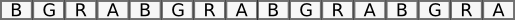
\includegraphics[scale=0.8]{imagenes/primerXmm.png}
\caption{Contenido del registro xmm al levantar de memoria cuatro pixeles}
\label{primerXmm}
\end{figure}

Luego utilizando la instrucción pshufb y una masara apropiada ordenamos su contenido para que quede como se muestra en la figura \ref{segundoXmm}

\begin{figure}[H]
\centering
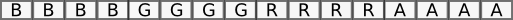
\includegraphics[scale=0.8]{imagenes/segundoXmm.png}
\caption{Contenido del registro xmm luego de utilizar la instruccion pshufb}
\label{segundoXmm}
\end{figure}

Utilizamos las instrucciones de desempaquetado de SIMD y un registro xmm lleno de ceros, para desempaquetar la parte alta y baja, obteniendo registros xmm con el contenido como se muestra en la figura \ref{tercerXmm}.


\begin{figure}[H]
\centering

\includegraphics[scale=0.8]{imagenes/tecerXmm.png}
\caption{Contenido resultante de desempaquetar parte alta y baja}
\label{tercerXmm}
\end{figure}

Luego volvemos a desempaquetar parte alta y baja de los dos registros obtenidos, y obtenemos cuatro registros xmm como se indica en la figura \ref{cuartoXmm}.


\begin{figure}[H]
\centering

\includegraphics[scale=0.8]{imagenes/cuartoXmm.png}
\caption{Contenido resultante de desempaquetar parte alta y baja nuevamente}
\label{cuartoXmm}
\end{figure}

Utilizando la instrucción cvtdq2ps convertimos los cuatro valores de los registros \ref{cuartoXmm}, excepto el que contiene los bytes de trasparencia(A), a tipo flotante. El objetivo es multiplicar cada color por value. Para hacer esto, previo al ciclo, utilizando la instrucción shufps, conseguimos en un registro xmm cuatro valores de tipo flotante con el valor que indica el índice de combinación de imágenes pasado por parametro, y en otro cuatro valores con 1-value tal como se indica en la figura \ref{value}.

\begin{figure}[H]
\centering

\includegraphics[scale=0.8]{imagenes/value.png}
\caption{Contenido de los registros utilizados para multiplicar por value los colores}
\label{value}
\end{figure}


Utilizando la instrucción de simd mulps, multiplicamos los colores transformados a tipo flotante por value.

Se repite el procedimiento para la segunda imagen, excepto que no se desempaqueta el byte de trasparencia(A), ya que solo interesa el byte de trasparencia de la primera imagen. En este caso multiplicamos por 1-value. Sumamos con la instruccion addps los valores obtenidos en la multiplicación, para los colores azul, verde y rojo. Luego convertimos a enteros de 32 bit, y con la instrucciones packusdw, y packuswb empaquetamos de forma que queden en un xmm los bytes en orden azul, verde, rojo y trasparencia. Este ultimo se consideran los bytes de la primera imagen almacenados en un registro xmm como se muestra la figura \ref{cuartoXmm}. Finalmente con la instrucción pshufb ordenamos los colores para que queden en el mismo orden en que ingresaron, y escribimos en memoria el resultado.

\subsubsection{Implementación en assembler 2}

Es analoga a la implementación anterior, pero en este caso se hacen la suma y multiplicación en numeros enteros. Se tiene en cuenta que la multiplicación de dos enteros, da como resultado un entero que puede ocupar el doble de tamaño. Para esto la para obtener el mismo resultado(aunque se pierdan decimales) es multiplicar a todo por 256, hacer las multiplicaciones en enteros y finalmente dividir por 256.

Antes de empezar el ciclo, multiplicamos en punto flotante 256 y value, y al resultado lo convertimos a enteros. En este proceso se pierden decimales. Como value es un numero entre cero y uno, al multiplicar por 256 y pasarlo a enteros, tenemos un valor entre 0 y 256, con lo que ocupa menos de un byte de tamaño. Utilizando la instrucción pshufb y una mascara, almacenamos en un registro xmm 8 replicas de este valor. Luego hacemos la resta en enteros entre 256 y el valor obtenido en la multiplicación. Nuevamente tenemos un valor entero entre 0 y 256 que entra en un byte, almacenamos 8 replicas del mismo en un registro xmm tal como se ve en la figura \ref{256value}. Estos registros seran utilizados para multiplicar los colores.

\begin{figure}[H]
\centering

\includegraphics[scale=0.8]{imagenes/256value.png}
\caption{Contenido de los registros utilizados para multiplicar en enteros}
\label{256value}
\end{figure}

El ciclo comienza igual que la implementación anterior, trayendo a un registro xmm 4 pixeles de la primer imagen desde memoria, ordenandolos con pshufb con una mascara para que queden como se indica en la figura~\ref{segundoXmm}. Utilizando punpcklbw y punpckhbw y un registro lleno de ceros obtenemos dos registros xmm, como pueden verse en a figura~\ref{tercerXmm}. Utilizando punpcklwd y psrldq, obtenemos finalmente tres registros xmm con el contenido tal como se indica en la figura~\ref{xmmAsm2}.

\begin{figure}[H]
\centering

\includegraphics[scale=0.8]{imagenes/xmmAsm2.png}
\caption{Contenido de los registros luego de hacer operaciones de desempaquetado}
\label{xmmAsm2}
\end{figure}


Utilizamos las instrucciones pmullw y pmulhuw para obtener las partes altas y bajas de la multiplicación de los colores(sin contar la transparencia) con el valor 256*value(convertido a entero) que se encuentra almacenado en un registro como se indica en la figura~\ref{256value}. Finalmente utilizamos la instrucción punpcklwd y punpckhwd para obtener el resultado final de la multiplicación. De esta manera realizamos multiplicaciones de enteros de 16 bit, con lo que obtenemos enteros de 32 bit. El registro que contiene los bytes de transparencia queda inalterado.

Se repite el procedimiento para la segunda imagen, pero sin guardar los bytes de transparencia. Dividimos los enteros por 256 utlizando un corrimiento a derecha de 8 bit con la instrucción "psrld xmm, 8". Y luego sumamos en enteros con las instrucciones paddd. Se decide dividir primero y luego sumar para evitar una posible saturación. Con las instrucciones packusdw y packuswb empaquetamos el resultado, de forma que queden en un xmm los bytes en orden azul, verde, rojo y trasparencia. Finalmente con la instrucción pshufb ordenamos los colores para que queden en el mismo orden en que ingresaron, y escribimos en memoria el resultado.

\newpage

\subsection{HSL}
El espacio RGB que usamos hasta ahora esta dado por un cubo donde cada componente corresponde a la intensidad de los colores primarios de la luz(rojo, verde y azul), para este filtro nos trasladamos al espacio HSL, este esta dado por tres componentes: HUE(color), Saturation(Saturación) y Lightness(Luminosidad). Este espacio se representa graficamente como un bicono donde cada punto esta determinado con: altura de la circunferencia a la que pertenece, radio de dicha circunferencia y ángulo dentro de la circunferencia, donde el color corresponde al ángulo, la saturacion al radio y la luminosidad a la altura.
El filtro consta de 3 etapas: (1)Transformación del espacio RGB a HSL del pixel, (2)suma de componentes y (3)transformacion del espacio HSL a RGB cuyas formulas son las siguientes:
\newline
\begin{enumerate}
	\item 
		H: \newline
		0 si $cmax = cmin$\newline
		$60 * ( (g-b)/d + 6 )$ si $cmax = r$\newline
		$60 * ( (b-r)/d + 2 )$ si $cmax = g$\newline
		$60 * ( (r-g)/d + 4 )$ si $cmax = b$\newline
		por ultimo si $h >= 360$ entonces $h = h - 360$\newline

		L: ( cmax + cmin ) / 510\newline

		S:\newline
		$0$ si $cmax == cmin$\newline
		$d / ( 1 - fabs( 2*l - 1 ) ) / 255.0001f$ caso contrario\newline
	  para este caso se debe dividir contra 255.0001f para evitar que s supere 1, evitando la propagación de errores.\newline

		Donde $cmax = max(b,g,r)$, $min = min(b,g,r)$ y $d = cmax - cmin$\newline
	
	\item 
		H:\newline
		$h + hh + 360$ si $h+hh >= 360$\newline
		$h + hh - 360$ si $h+hh < 0$\newline
		$h + hh$ caso contrario\newline

		S:\newline
		0 si $s+ss < 0$\newline
		1 si $s+ss >= 1$\newline
		$s + ss$ caso contrario\newline

		L:\newline
		0 si $l+ll < 0$\newline
		1 si $l+ll >= 1 $\newline
		$l+ll$ caso contrario\newline

		donde hh, ll y ss son valores pasados por parametro
		\newpage

	\item
		RGB:\newline
			r=c g=x b=0 si $0<=h$ y $h<60$\newline
			r=x g=c b=0 si $60<=h$ y $h<120$\newline
			r=0 g=c b=x si $120<=h$ y $h<180$\newline
			r=0 g=x b=c si $180<=h$ y $h<240$\newline
			r=x g=0 b=c si $240<=h$ y $h<300$\newline
			r=c g=0 b=x si $300<=h$ y $h<360$\newline

		Escala:\newline
		$b = (b+n) * 255$\newline
		$g = (g+n) * 255$\newline
		$r = (r+n) * 255$\newline

		donde:\newline
		$c = ( 1 - fabs( 2*l - 1 )) * s;$\newline
		$x = c * ( 1 - fabs( fmod( h/60, 2 ) - 1 ) )$\newline
		$m = l - c / 2$\newline


\end{enumerate}

\subsubsection{Implementacion en assembler 1}
OBS: Para esta implementación usamos dos funciones provistas por la catedra(rgbTOhsl | hslTOrgb) y nos concentramos en (2), donde el algoritmo general va a recorrer la imagen como si fuera un vector, tomando pixel por pixel, transformandolo a HSL, luego procesandolo y finalmente transformandolo a RGB para devolverlo a memoria(para mas información sobre otras posibles implementaciones ver sección 3).



Recibimos como parametros una imagen representada en memoria de la misma manera que en los anteriores filtros, ancho, alto y tres valores hh, ss y ll, los cuales modificaran los 3 elementos de la representacion HSL del pixel.
Primero acomodamos los datos de entrada de manera que nos queden dentro de un registro xmm, dado que cada dato ocupa 16bits los acomodaremos de manera tal que los 3 elementos queden empaquetados.

\begin{figure}[H]
\centering
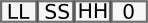
\includegraphics[scale=0.8]{imagenes/llsshh.png}
\caption{Organizacion de valores de entrada}
\label{lshValue6}
\end{figure}

A continuación movemos a un registro xmm el valor que usaremos como limite superior de la suma para h por un lado y s y l por otro ya que las modificaciones seran diferentes para los dos casos, como limite inferior simplemente colocaremos 0 en un registro usando pxor.



Dado que la imagen está representada linealmente en memoria vamos a recorrerla como un vector dentro de un ciclo principal que se movera de a un pixel. Una vez dentro del ciclo procecedemos a llamar a rgbTOhsl y movemos el pixel resultante a un registro xmm.

\begin{figure}[H]
\centering
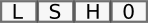
\includegraphics[scale=0.8]{imagenes/lsh.png}
\caption{Contenido del registro XMM}
\label{lshValue5}
\end{figure}

Ahora sumamos los valores hsl con los que teniamos como parametro con addps(a) para luego revisar los limites.

\begin{figure}[H]
\centering

\includegraphics[scale=0.8]{imagenes/sumahsl.png}
\caption{Contenido del registro XMM}
\label{lshValue4}
\end{figure}

Para realizar las comparaciones correspondientes primero generamos los vectores que sumados o restados nos den los resultados que queremos en cada caso, para esto tomamos por un lado un registro con el valor 360(b) en la posicion de h y procedemos al primer caso de h, para esto aplicamos cmpleps para crear una mascara(c) en donde si h es mayor a 360 nos quedaran 1s en los valores donde se deberia ubicar h o 0s en caso contrario, luego aplicamos pand usando (b) y (c) para finalmente restarlo a (a), dando como resultado h + hh ó h + hh - 360 dependiendo del caso, a continuacion veremos como se aplica esta idea a s y a l.

\begin{figure}[H]
\centering
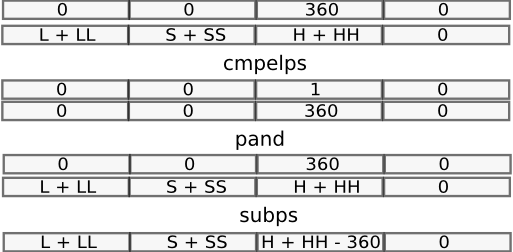
\includegraphics[scale=0.8]{imagenes/caso1hsumahsl.png}
\caption{ejemplo de estados usando cmp y and para el caso h mayor a 360}
\label{lshValue3}
\end{figure}

Para s y l, como su resultado debe ser 1 en caso de pasar el limite, simplemente colocamos s+ss-1 y l+ll-1 empaquetados en un registro aparte pero en las mismas posiciones que s+ss y l+ll respectivamente, luego aplicamos la misma idea que en la figura 10 pero comparando contra 1 en lugar de 360 y finalmente sumando s+ss-1 o l l+ll-1 según corresponda para lograr que quede 1 ó s+ss/l+ll en los valores finales. Los casos de los limites inferiores que se realizan inmediatamente despues en el codigo son analogos pero comparando contra 0s, dando una sucesion de estados con la cual al llegar al final, (1) tendra los valores l+ll ó 1 ó 0, s+ss ó 1 ó 0,  h+hh ó h+hh+360 ó h+hh-360 y 0 respectivamente en sus posiciones empaquetadas.

\subsubsection{Implementación en assembler 2}
Para esta implementación reutilizamos el codigo de la primera y nos concentramos en implementar (1) y (3), cuyas reglas son las siguientes:
\newline\newline
reglas.....
\newline\newline
Transformación del espacio RGB a HSL
\newline\newline
Como parametros tenemos el puntero al pixel de la matriz que queremos convertir y un vector de floats donde guardar la version hsl del pixel.
Primero levantamos el pixel a un registro de proposito general y lo movemos de a bytes a otros registros para separar los elementos RGBA del pixel, como cada uno ocupa 1B  simplemente movemos entre registros de 1B y luego shifteamos al que contiene todo el pixel 1B a la derecha hasta que queden todos separados.
\newline
A continuacion pasamos a calcular el maximo entre RGB, para esto acumulamos uno de los tres valores y comparamos contra los otros acarreando siempre al mayor, analogamente para calcular el minimo.
\newline
Luego calculamos D, para esto simplemente colocamos el maximo en otro registro y le restamos el minimo.
\newline
Despues calculamos H, para esto separamos los casos posibles en donde simplemente seteamos los registros que luego seran operados, esto se logra comparando el maximo contra los posibles valores, saltando, seteando los registros segun los valores que les correspondan, convirtiendolos en valores de punto flotante con cvtdq2ps y finalmente utilizando subps, divps, addps y mulps para llegar a la formula que les corresponda.
\newline

\begin{figure}[H]
\centering

\includegraphics[scale=0.8]{imagenes/resultH.png}
\caption{(contenido del registro xmm al final del caso 3, para mas informacion sobre los casos ver el codigo fuente)}
\label{lshValue}
\end{figure}

 por ultimo revisamos que no haya caido fuera de rango, para esto aplicamos la misma técnica que en la primera implementacion usando una comparacion y luego aplicando pand y subps para llegar a h ó h-360.
 \newline
Ahora calculamos L, para esto tomamos el maximo y le sumamos el minimo, lo pasamos a un registros xmm, lo convertimos y aplicamos una division contra una posicion en memoria que contiene 510.
\newline
Por ultimo queda calcular S, en caso de que sea igual al minimo simplemente lo seteamos en 0, caso contrario pasamos a efectuar las cuentas. Movemos d a un registro xmm y lo convertimos a punto flotante, luego usamos addps, mulps y subps para llegar a 2*l - 1 donde aplicamos pand contra una mascara que contiene todos 1 excepto en el bit mas significativo, de esta manera seteamos en 0 el bit de signo de la representación del float que contiene 2*l - 1, convirtiendolo en abs(2*l - 1). Finalmente dividimos a d por abs(2*l - 1) y luego por 255.0001 desde una direccion en memoria que lo contiene.
\newline

\begin{figure}[H]
\centering

\includegraphics[scale=0.8]{imagenes/representacionfloat.png}
\caption{Representación del punto flotante en memoria}
\label{lshValue2}
\end{figure}

Terminado lo anterior procedemos a empaquetar los datos con punpckldq de manera que dentro del registro quede LHSA para que cuando lo volquemos a memoria sea de la forma ASHL.
\newline\newline

Transformación del espacio HSL a RGB
\newline\newline

Como parametros tenemos un vector de floats donde se encuentra la version hsl del pixel y el puntero al pixel de la matriz donde queremos colocar su version RGB. Primero levantamos el pixel a un registro xmm y separamos sus componentes entre otros registros xmm usando punpckldq, punpckhdq, psrldq y pslldq.
\newline
Luego calculamos C, para esto levantamos de memoria un 1 a un registro xmm y pasamos a realizar las cuentas usando addss, mulss y subss hasta llegar a 2*l-1 donde aplicamos pand contra una mascara de la misma que en la transformacion anterior para lograr abs(2*l - 1), luego le restamos a 1 el resultado y lo multiplicamos por S.
\newline
A continuación calculamos X, para esto pasamos el valor 60 a un registro xmm, lo convertimos a float y dividimos H por 60, luego para calcular fmod(h/60, 2), simplemente restamos 60 hasta que el numero sea menor a 2 ya que como el primer operando es h/60, ese numero estara entre 0 y 60, como siguiente operacion resto y aplico la misma idea de mascara para lograr abs(fmod(h/60, 2) - 1) y finalmente resto 1 y multiplico por C.
\newline
En este punto nos queda calcular M y luego ordenar lo que ya calculamos, empecemos con lo primero. Simplemente copio el valor C a otro registro, lo dividimos por dos y se lo restamos a l.
\newline
Ahora vamos a calcular RGB, en esta parte nos dedicamos a ver a que valor(r, g o b) corresponden X y C respectivamente, para esto preguntamos linealmente, aumentando de a 60 en que caso cae H, sumandole 60 y comparando contra H con comiss para luego efectuar un jb de ser necesario. Dentro de cada caso se tiene un registro xmm que contiene a c y un registro de proposito general que contiente a X y, dependiendo del caso, se shiftea c hasta el lugar que corresponda a la componente a la que debe ir y luego se aplica pinsrd para insertar X en la posicion que le corresponda.
\newline
Finalmente nos queda calcular la escala, para esto primero colocamos M en un registro xmm, lo shifteamos y sumamos con pslldq y addps contra m hasta que queden tres valores iguales empaquetados en la posiciones donde deben ir r, g y b, a continuacion se suma este registro con addps al que contenia a C y X y se lo multiplica por 255 contra un registro que previamente habia levantado ese valor de memoria, para lograr (X + m) * 255 en cada una de las componentes. Luego se inserta A en la ultima posicion y se convierte a entero truncando el valor, se tomo esta decisión ya que la conversión normal redondeaba al entero más cercano.
\newline
Para ordenar los datos(ya que deben tener 1B cada uno y a esta altura tienen 4B) aplicamos pshufb sobre el registro que contiene RGBA para pasar dichos valores a 1B(tomando solo el primer byte de estos) en sus posiciones finales y luego moverlo a memoria(figura 14).

\begin{figure}[H]
\centering
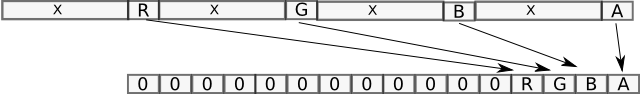
\includegraphics[scale=0.8]{imagenes/shufle.png}
\caption{Uso de pshufB}
\label{lshValue}
\end{figure}



\section{Experimentación}

Se llevaron a cabo experimentos para comparar el tiempo de computo de las distintas versiones de los filtros, en assembler y en C, con distintas optimizaciónes. Se estudio el tiempo de computo para distintos parámetros de los filtros, y utilizando distintos conjuntos de imágenes: Normal(incluyen todos los colores), Black(imágenes negras), White(imágenes blancas).


\subsection{Blur}

En las siguientes figuras encontramos los resultados obtenidos para el filtro blur:

\begin{figure}[H]
	\minipage{0.5\textwidth}
	\begin{center}
		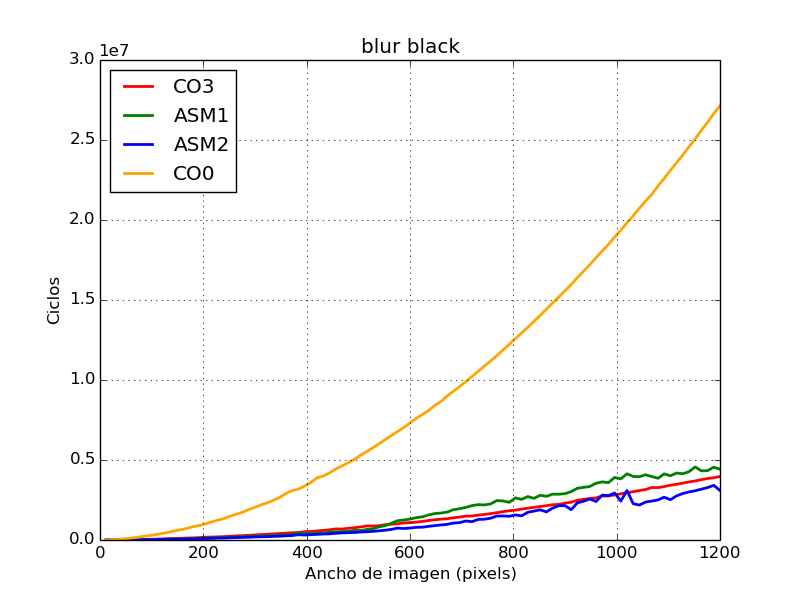
\includegraphics[scale=0.4]{../tp2-bundle.v2/Testing/plots/all/blur-black--all.png}
		\caption{Rendimiento del filtro blur para imágenes negras}
		\label{fig:exp1-5}
	\end{center}
	\endminipage\hfill
	\minipage{0.5\textwidth}
	\begin{center}
		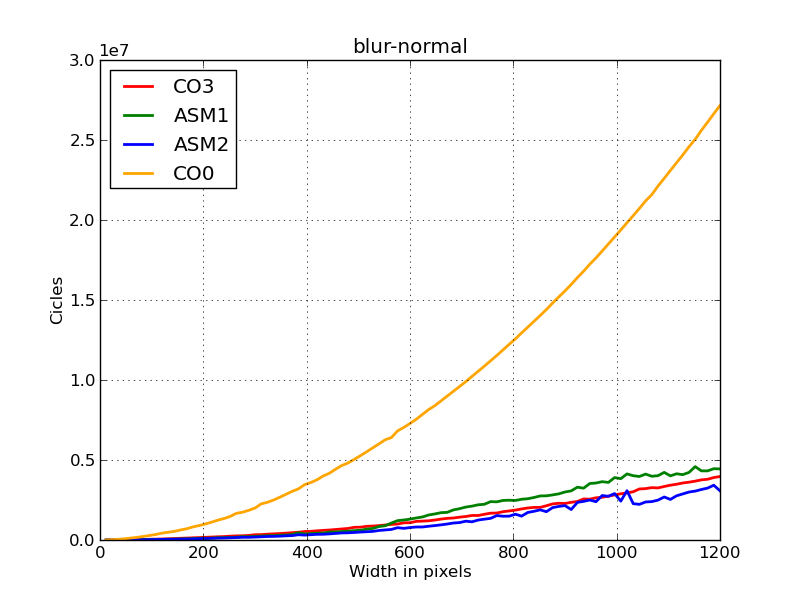
\includegraphics[scale=0.4]{../tp2-bundle.v2/Testing/plots/all/blur-normal--all.png}
		\caption{Rendimiento del filtro blur para imágenes normales.}
		\label{fig:exp1-2}
	\end{center}
	\endminipage\hfill
\end{figure}
\begin{figure}[H]
	\begin{center}
		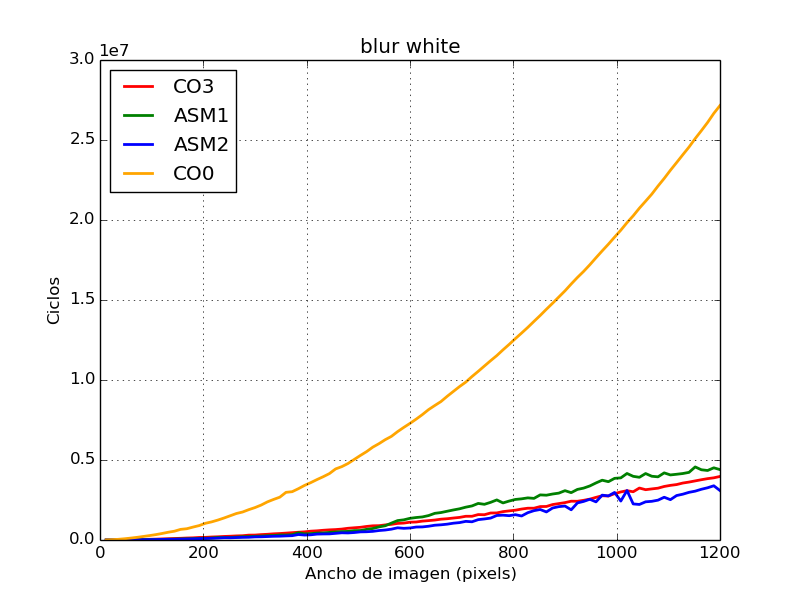
\includegraphics[scale=0.4]{../tp2-bundle.v2/Testing/plots/all/blur-white--all.png}
		\caption{Rendimiento del filtro blur para imágenes blancas.}
		\label{fig:exp1-1}
	\end{center}
\end{figure}



Las dos implementaciones en assembler, utilizan una memoria temporal del tamaño de la imagen para ir almacenando los resultados parciales. Como trabajamos con imágenes pequeñas, esto no resulta costoso, pero podria ser evitado con un algoritmo mas complejo.

La segunda implementación en assembler en comparación con la primera resulta tener un rendimiento un poco mejor. Esto se debe a que esta ultima realiza tres lecturas de memoria y una escritura para escribir en la memoria temporal un pixel, en cambio la segunda utiliza cuatro lecturas y cuatro escrituras de memoria para escribir en la memoria temporal cuatro pixeles. Esta ultima podria ser mejorada para que con una escritura escribir los cuatro pixeles en memoria, en lugar de hacerlo con accesos separados.

La implementacion en C sin optimización resulta ser mucho mas costosa que las otras, lo cual se puede deber a que por cada color realiza una suma y un acceso a memoria, lo que implica una cantidad de accesos a memoria muy grande. La implementación en C optimizada resulta tener un rendimiento mejor que una version de assembler, pero peor que el otro.






Al no tener saltos condicionales, obtenemos el mismo rendimiento para los distintos tipos de imágenes. 


\subsection{Merge}

En las siguientes figuras encontramos los resultados obtenidos para el filtro merge:

\begin{figure}[H]
	\minipage{0.5\textwidth}
	\begin{center}
		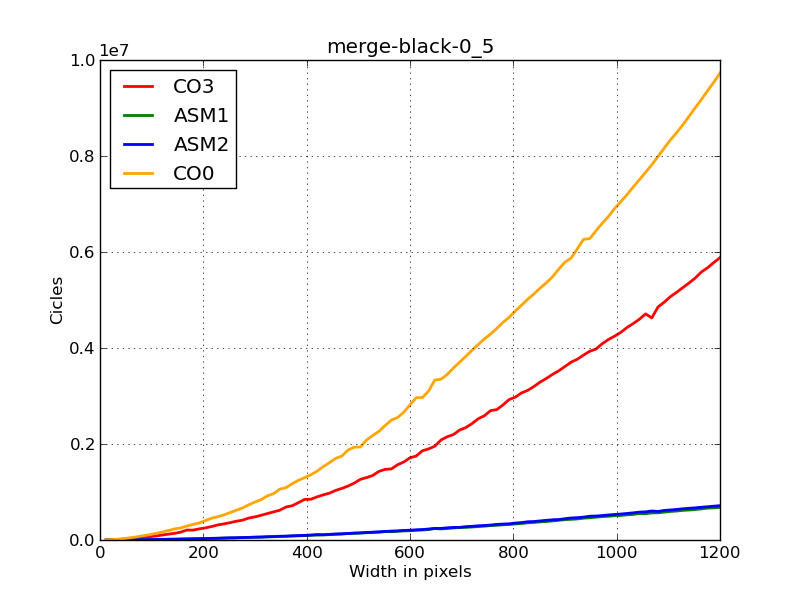
\includegraphics[scale=0.4]{../tp2-bundle.v2/Testing/plots/all/merge-black-05--all.png}
		\caption{Rendimiento para un value de 0.5, imágenes negras.}
		\label{fig:exp1-5}
	\end{center}
	\endminipage\hfill
	\minipage{0.5\textwidth}
	\begin{center}
		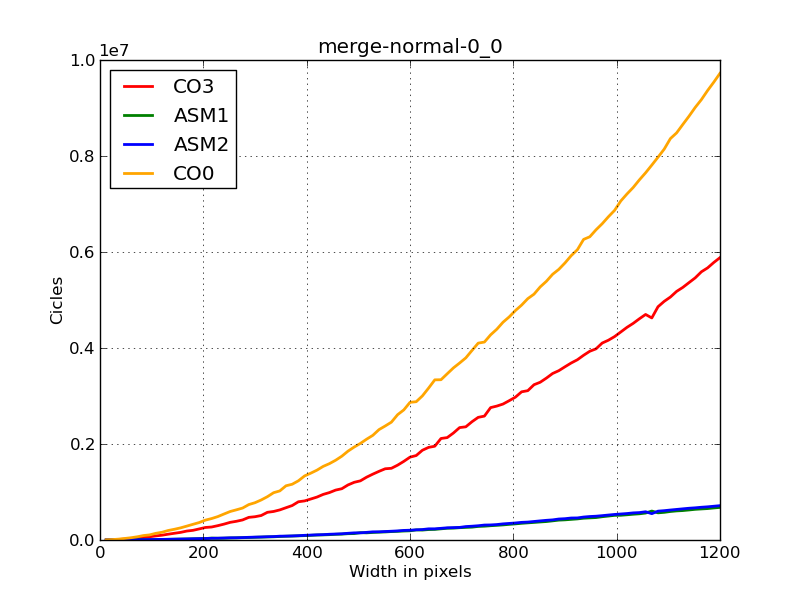
\includegraphics[scale=0.4]{../tp2-bundle.v2/Testing/plots/all/merge-normal-00--all.png}
		\caption{Rendimiento para un value de 0.0, imágenes normales.}
		\label{fig:exp1-2}
	\end{center}
	\endminipage\hfill
\end{figure}
\begin{figure}[H]
	\minipage{0.5\textwidth}
	\begin{center}
		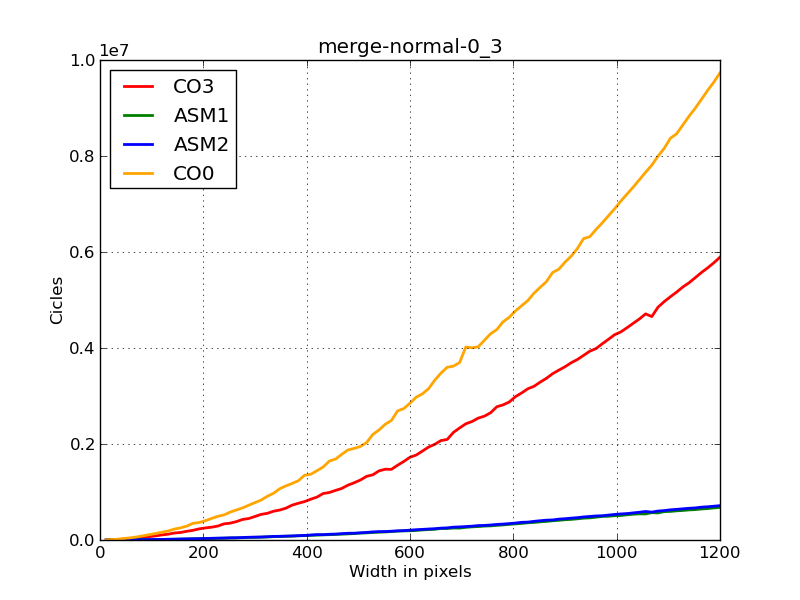
\includegraphics[scale=0.4]{../tp2-bundle.v2/Testing/plots/all/merge-normal-03--all.png}
		\caption{Rendimiento para un value de 0.3, imágenes normales.}
		\label{fig:exp1-1}
	\end{center}
	\endminipage\hfill
	\minipage{0.5\textwidth}
	\begin{center}
		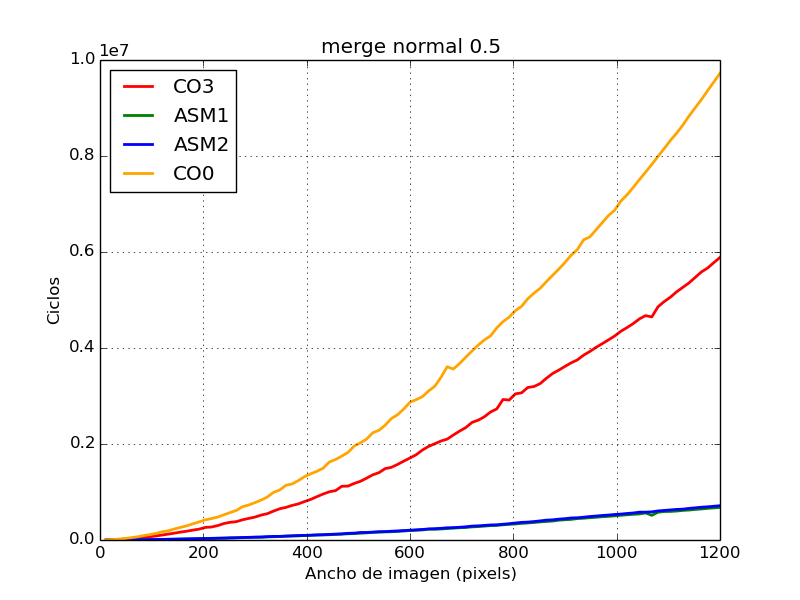
\includegraphics[scale=0.4]{../tp2-bundle.v2/Testing/plots/all/merge-normal-05--all.png}
		\caption{Rendimiento para un value de 0.5, imágenes normales.}
		\label{fig:exp1-0.5}
	\end{center}
	\endminipage\hfill
		\minipage{0.5\textwidth}
	\begin{center}
		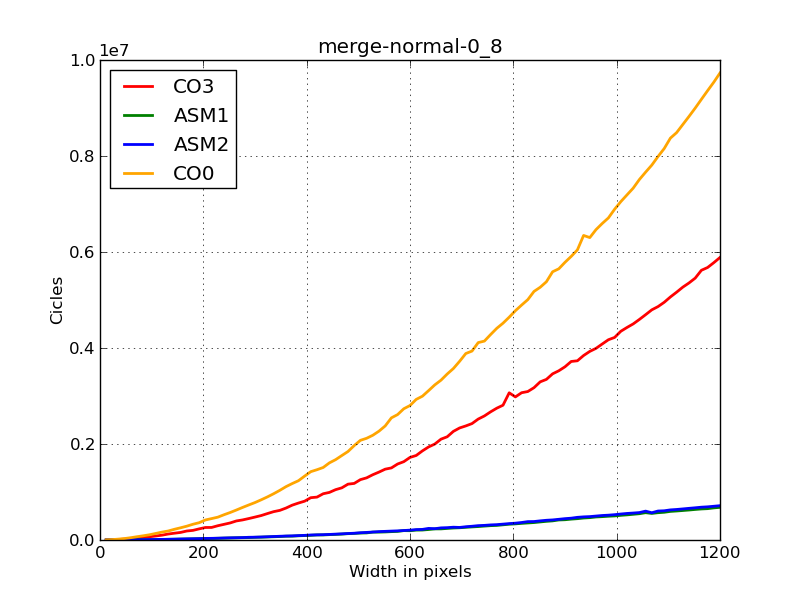
\includegraphics[scale=0.4]{../tp2-bundle.v2/Testing/plots/all/merge-normal-08--all.png}
		\caption{Rendimiento para un value de 0.8, imágenes normales.}
		\label{fig:exp1-0.5}
	\end{center}
	\endminipage\hfill
		\minipage{0.5\textwidth}
	\begin{center}
		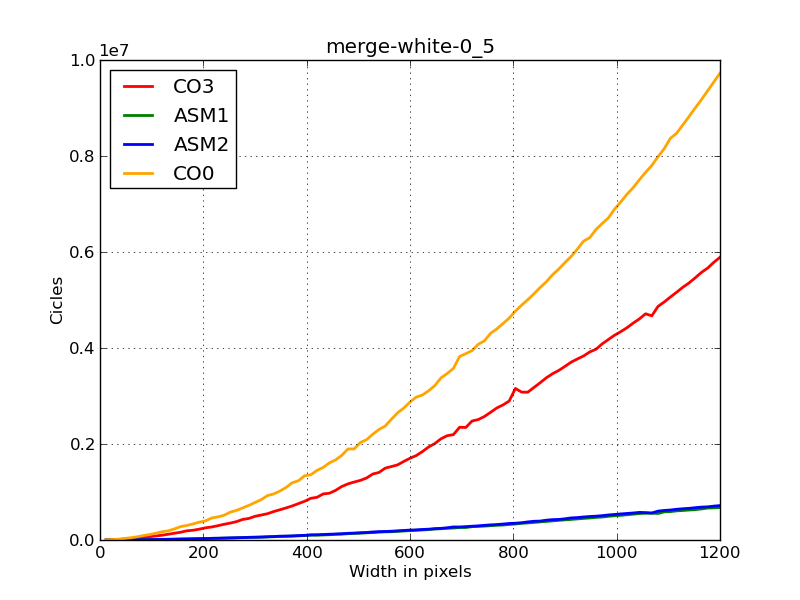
\includegraphics[scale=0.4]{../tp2-bundle.v2/Testing/plots/all/merge-white-05--all.png}
		\caption{Rendimiento para un value de 0.5, imágenes blancas.}
		\label{fig:exp1-0.5}
	\end{center}
	\endminipage\hfill
\end{figure}

Podemos ver que la implementación en C tiene un rendimiento menor, aun utilizando un compilador que optimiza. Esto se debe a que la imágenes se encuentran almacenadas en memoria en forma de matrices de pixeles, en la implementación en assembler se traen desde memoria cuatro pixeles a un registro xmm, a diferencia la implementacion en C, en la cual se hace un acceso a memoria por color. Con lo que la cantidad de accesos a memoria es mucho menor en la implementación en assembler, lo que implica un tiempo de computo mucho menor. Además en la implementación en assembler, utilizando las instrucciones simd se hacen multiplicaciones y sumas de a cuatro colores, a diferencia de la C, en la estas operaciones se hacen color por color.

Tanto las implementaciones en C como en assembler de este filtro presentan el mismo rendimiento para los distintos tipos de imágenes, y solo dependen de la cantidad de pixeles a procesar. Esto se debe a que ambas implentaciones no presentan saltos condicionales.

Para las implementaciones en assembler, no se aprecia una diferencia significativa en el tiempo de computo al operar con enteros o con floats. La imagen resultante para enteros tiene un error un poco mayor, pero esta diferencia no es apreciable a simple vista.

Cuando la cantidad de pixeles a procesar es grande, la diferencia de tiempo de computo entre la implementación en C y su version en assembler.








\section{Conclusiones y trabajo futuro}


\end{document}

